\section{Expectation and Variance}
\subsection{1-dimensional Random Variables}
Expectation is the averaging operation carried out over the outcomes $\omega$ in $\Omega$ according to their respective probabilities.\\

Consider the example of a continuous random variable $X$ with probability density function $f_X(x)$. Then the {\elevenit Mean}, $\mu$, is given by $$\mu = E[X] = \int_{-\infty}^{\infty}\, x f_X(x) dx$$ in which case $E[X]$ is just the definition of the mean value of X. This concept can be extended to functions of the random variable $X$, i.e., g(X) and we find that $$E[g(X)] = \int_{-\infty}^{\infty}\, g(x) f_X(x) dx.$$ This result is intuitively reasonable but needs to be proven also from the definition of the averaging method over the random variable $Y = g(X)$.\\

The {\elevenit Variance}, $\sigma^2$, is given by  $$\sigma^2 = \hbox{Var}[X] = E[(X - E[X])(X- E[X])]\, = E[X^2] - (E[X])^2.$$ Since $\mu = E[X]$, this result can also be written as $$\sigma^2 = E[X^2] - \mu^2.$$

If one has two random variables $X$ and $Y$ then we will distinguish the respective means by $\mu_X = E[X]$ and $\mu_Y = E[Y]$ and define the {\elevenit Covariance} by Cov[Y,Y] which is given by 
$$\hbox{Cov}[X,Y] = E[(X-E[X])(Y-E[Y])] = E[(X - \mu_X)(Y-\mu_Y)].$$

For a Gaussian random variable $X$, let us compute $E[X]$: 
$$E[X] = {1\over \sqrt{2\pi}\sigma} \int_{-\infty}^{\infty}\, x e^{-(x-\mu)^2/2\sigma^2}\, dx$$
Making the substitution $u = (x -\mu)/\sigma, du = dx/\sigma, E[X]$ becomes 
\begin{eqnarray*} E[X] &=& {1\over \sqrt{2\pi}\sigma} \int_{-\infty}^{\infty}\, (\sigma u + \mu) e^{-u^2/2}\, \sigma du \\
      &=& {1\over \sqrt{2\pi}} \int_{-\infty}^{\infty}\, (\sigma u + \mu) e^{-u^2/2}\, du\\
      &=& \sigma {1\over \sqrt{2\pi}} \int_{-\infty}^{\infty}\, u e^{-u^2/2}\, du + \mu {1\over \sqrt{2\pi}} \int_{-\infty}^{\infty}\, e^{-u^2/2}\, du\\
\end{eqnarray*}

Now, the first term has an anti-derivative given by $${d\over du}(-e^{-u^2/2}) = u e^{-u^2/2}$$ and therefore  $$ \int_{-\infty}^{\infty}\, u e^{-u^2/2}\, du = -e^{-u^2/2}\big|_{-\infty}^{\infty} = 0$$
Also using Eq. [\ref{eqn:gaussnormalization}] the integral multiplying $\mu$ is equal to $1$ and therefore $E[X] = \mu$.\\

The Moment Generating Function (m.g.f. see Section[\ref{sec:generating}] for more details) for the $N(\mu, \sigma^2)$ Gaussian random variable is defined by
$$\psi(u) = E[e^{uX}]$$
Using the probability density function for a $N(\mu, \sigma^2)$ we have 
\bearray \psi(u) 
&=& {1\over \sqrt{2\pi} \sigma} \int_{-\infty}^\infty e^{\big( -{(x-\mu)^2\over 2\sigma^2} \big)}\, e^{xu}\, dx \\
&=& {1\over \sqrt{2\pi} \sigma} \int_{-\infty}^\infty e^{\big(-{(x-\mu)^2\over 2\sigma^2} + xu \big)}\, dx
\eearray
Using the substitution $y = x -\mu$ we have 
\be \psi(u)  = e^{\mu u}{1\over \sqrt{2\pi} \sigma} \int_{-\infty}^\infty e^{\big(-{y^2\over 2\sigma^2} + \mu y \big)}\, dy \label{eqn:GaussianMomentGeneratingFunction}\ee
From an integral table we find the Gaussian integral formula, viz., 
\be\int_{-\infty}^\infty e^{(-ay^2 + by)}\, {dy\over 2\pi} = {1\over\sqrt{4\pi a}}\,e^{b^2/4a}\label{eqn:GaussianIntegral}\ee
Using Eq. [\ref{eqn:GaussianIntegral}] in Eq. [\ref{eqn:GaussianMomentGeneratingFunction}] we obtain the m.g.f for an $N(\mu, \sigma^2)$ random variable:
\be \psi(u) = \exp\big\{\sigma^2u^2/2 + \mu u\big\} \ee
Taking the derivative of $\psi(u)$ with respect to $u$ we find $$\psi'(u) = (\mu + u \sigma^2)\exp\{\sigma^2 u^2/2 + \mu u\}.$$
The relationship between the derivative of the m.g.f and the first moment of the respective random variable, $E[X]$ can be obtained by setting evaluating $\psi'(0)$ and we see $$E[X] = \psi'(0) = \mu.$$

We can use the m.g.f. also to obtain the second moment as well and find

$$ \psi''(u) = (\mu + u \sigma)^2 \exp\{\sigma^2 u^2/2 + \mu u\}  + \sigma^2 \exp\{\sigma^2 u^2/2 + \mu u\}$$ and therefore $E[X^2] = \psi''(0) = \mu^2 + \sigma^2$. \\
 
To find the variance of the Gaussian random variable we have to compute the second moment about the mean or  $$\hbox{Var}[X] = E[(X-(E[X])^2] = E[X^2] - (E[X])^2 = \mu^2 + \sigma^2 - \mu^2 = \sigma^2.$$

The m.g.f. can also be defined with respect to $(X-\mu)$. $$\psi_{(X-\mu)}(u) = E[e^{u(X-\mu)}] = \exp\{\sigma^2 u^2/2\}$$ which is the same functional form as $\psi(u)$ and depends only on the parameter $\sigma^2$. This means that all the central moments, $E[(X-\mu)^n]$ are functions only of $\sigma^2$. Let $\psi^{(n)}(u) \equiv {d^n\over du^n}\, \psi(u)$. Then we can show that
$$\psi^{(n+2)}(0) = (n-1)\sigma^2 \psi^{(n)}(0).$$ With the initial condition $\psi^{(1)}(0) = 0$, (first central moment), it immediately follows that $\psi^{(n)}(0) = 0$ for all odd $n\ge1$. With the initial conditions $\psi^{(0)}(0) = 1$, we have 

\begin{equation}\psi^{(n)}(0) = 1\cdot3\cdot5 \hdots (n-1)\, \sigma^n = \{(n-1)!!\} \sigma^n \quad\quad \hbox{for all even $n\ge2$.}\label{eqn:moments}\end{equation}
%\begin{equation}\psi^{(n)}(0) = 1\cdot3\cdot5 \hdots (n-1)\, \sigma^n \quad\quad \hbox{for all even $n\ge2$.}\label{eqn:moments}\end{equation}

\subsection{Multi-dimensional Random Variables}
In dealing with more than one random variable, the concept of joint probability distribution arises. The continuous random variables $X_1, X_2, ... , X_n$ are said to be {\elevenit jointly distributed} if they are defined on the same probability space. They may be characterized by their {\elevenit joint distribution function} or {\elevenit cummulative distribution function}:
$$F_{X_1, X_2, ..., X_n}(x_1, x_2, ..., x_n) = \hbox{Probability}\{x_1(\omega) \le x_1, x_2(\omega) \le x_2,\hdots,x_n(\omega)\le x_n \},$$ where 
$$\{ x_1(\omega), ..., x_n(\omega) \le x_n\} = \{x_1(\omega) \le x_1\} \cap \{x_2(\omega)\le x_2\} \cap ... \cap \{x_n(\omega)\}$$ or alternatively by their {\elevenit joint density function}
$$F_{X_1, X_2, ..., X_n}(x_1, x_2, ..., x_n) = \int_{-\infty}^{x_1}\, ... \int_{-\infty}^{x_n} f_{X_1, ..., X_n}(\xi_1, ..., \xi_n) \, d\xi_1 ... d\xi_n.$$

It follows that the joint density function is related to the joint distribution function by 
$$f_{X_1, ..., X_n}(x_1, ..., x_n)  = {\partial^n \over \partial x_1, \partial x_2, ... \partial x_n} F_{X_1, X_2, ..., X_n} (x_1, x_2, ..., x_n)$$
 
The joint density function can be used to define the probability distribution for a vector of random numbers. Consider such a vector ${\bf X}$:\\

$${\bf X} =  
\begin{bmatrix}
           X_{1} \\
           X_{2} \\
           \vdots \\
           X_{n}
\end{bmatrix}$$

The matrix transpose of ${\bf X}$  is denoted by $${\bf X}^T  = (X_1, X_2, \hdots, X_n)$$

Now for $j,k = 1, 2, \hdots, n$ let $$m_j = E[X_j], \quad\quad K_{jk} = \hbox{Cov}[X_j, X_k].$$ \\
Let  the matrix of covariances be given by
$${\bf K} = 
\begin{bmatrix}
K_{11} & K_{12} & \hdots K_{1n} \\
K_{21} & K_{22} & \hdots K_{2n} \\
\vdots  \\
K_{n1} & K_{n2} & \hdots K_{nn} \\
\end{bmatrix}$$

and let the inverse matrix be represented by 

$${\bf K}^{-1} = 
\begin{bmatrix}
K^{11} & K^{12} & \hdots K^{1n} \\
K^{21} & K^{22} & \hdots K^{2n} \\
\vdots  \\
K^{n1} & K^{n2} & \hdots K^{nn} \\
\end{bmatrix}$$

Now the $n$ random variables $X_1, \hdots X_n$ are jointly normally distributed if their joint probability density, for any real numbers $x_1, \hdots x_n$, is given by

$$f_{X_1, ..., X_n}(x_1, ..., x_n)  = {1\over(2\pi)^{n/2}} {1\over|K|^{1/2}} \exp\big\{ - {1\over2}\sum_{j,k = 1}^n (x_j - m_j) K^{jk} (x_k-m_k)\big\}$$where $|K|$ is the determinant of the ${\bf K}$ matrix (i.e., $|K| = \det {\bf K}$).\\

Let 
$${\bf m} =
\begin{bmatrix}
           m_{1} \\
           m_{2} \\
           \vdots \\
           m_{n}
\end{bmatrix}
\quad \quad {\bf x} = 
\begin{bmatrix}
           x_{1} \\
           x_{2} \\
           \vdots \\
           x_{n}
\end{bmatrix}
$$ \\

Using matrix multiplication we can also express the joint probability distribution more succiently as 

\be f_{X_1, ..., X_n}(x_1, ..., x_n)  = {1\over(2\pi)^{n/2}} {1\over|K|^{1/2}} \exp\big\{ - {1\over2} ({\bf x} - {\bf m})^T {\bf K}^{-1} ({\bf x} -{\bf m})\big\}. \label{eqn:GaussianDistribution}\ee

The quantity $$D_M({\bf x}, {\bf y}) = \sqrt{({\bf x} - {\bf y})^T {\bf K}^{-1} ({\bf x} -{\bf y})}$$ is known in statistics as the  ``Mahalanobis distance'' \cite{Mahalanobis} and it measures the separation between ${\bf x}$ and ${\bf y}$. The argument of the exponential in Eq. [\ref{eqn:GaussianDistribution}] involves $D^2_M({\bf x},{\bf m})$.\\

The m.g.f. for a $n$-vector Gaussian random variable $X$ defined by the above ${\bf m}$ and ${\bf K}$ matrices is given by 
(Theorem [\ref{thm:mgfMultivariateGaussian}] in Section [\ref{sec:generating}])
$$\psi_X({\bf u}) = \exp\{ {\bf u}^T{\bf m} + {1\over2}{\bf u}^T{\bf K u} \}, $$ where ${\bf u}$ is an $n$-vector. \\

If a linear transformation is performed on a vector of Gaussian random variables, then the transformed random variable also is a multivariate Gaussian.
\begin{theorem}
\label{thm:Gaussian}
Let the $n$-vector random variable $Z \sim N(m_z, K_z)$. Let $W = CZ + a$ where $C$ is a $q\times n$ constant matrix, $a$ is a constant $q$-vector, and $W$ is a random $q$-vector. Then $W \sim N(Cm_z + a, CK_zC^T)$.  
\end{theorem}
\begin{proof}
Write the m.g.f. for $W$
\begin{eqnarray*}
\psi_W({\bf u}) &=& E[\exp[{\bf u}^T{\bf w}] = \exp({\bf u}^T{\bf a}) E[\exp({\bf u}^T{\bf C}{\bf z})] \\
&=& \exp[{\bf u}^T{\bf w}] = \exp({\bf u}^T{\bf a}) \psi_Z({\bf C}^T{\bf z}) 
\end{eqnarray*}
But $Z$ is Gaussian, so that  (see Theorem [\ref{thm:mgfMultivariateGaussian}] )
$$\psi_Z({\bf u}) = \exp\{ {\bf u}^T({\bf C m_z}) + {1\over2}{\bf u}^T{\bf C K_z}{\bf C}^T{\bf u} \}$$
Therefore 
$$\psi_W({\bf u}) = \exp\{ {\bf u}^T({\bf C m_z} + {\bf a})  + {1\over2}{\bf u}^T[{\bf C K_z}{\bf C}^T]{\bf u} \}\qed$$
\end{proof}

\subsection{Jensen's Inequality}
Jensen's inequality generalizes the statement that the secant line of a convex function lies {\elevenit above}\/ the graph of the function, 
which is Jensen's inequality for two points: the secant line consists of weighted means of the convex function (for $t \in [0,1]$),
$$t f(x_{1}) + (1-t) f(x_{2}),$$ while the graph of the function is the convex function of the weighted means,
$$f\left(tx_{1}+(1-t)x_{2}\right).$$
Thus, Jensen's inequality is $${\displaystyle f\left(tx_{1}+(1-t)x_{2}\right)\leq tf(x_{1})+(1-t)f(x_{2}).}$$
In the context of probability theory, it is generally stated in the following form: if X is a random variable and $\phi$ is a convex function, then
$${\displaystyle \varphi \left(\operatorname {E} [X]\right)\leq \operatorname {E} \left[\varphi (X)\right].}$$
The difference between the two sides of the inequality, 
${\displaystyle \operatorname {E} \left[\varphi (X)\right]-\varphi \left(\operatorname {E} [X]\right)}, $ is called the Jensen gap. 
\clearpage
A graphical demonstration of Jensen's inequality for convex functions is shown in Fig. \ref{fig:Jensen}
\begin{figure}[hb]
%\epsfysize=6cm %%%% whatever vertical size you want in cm or inches
\center{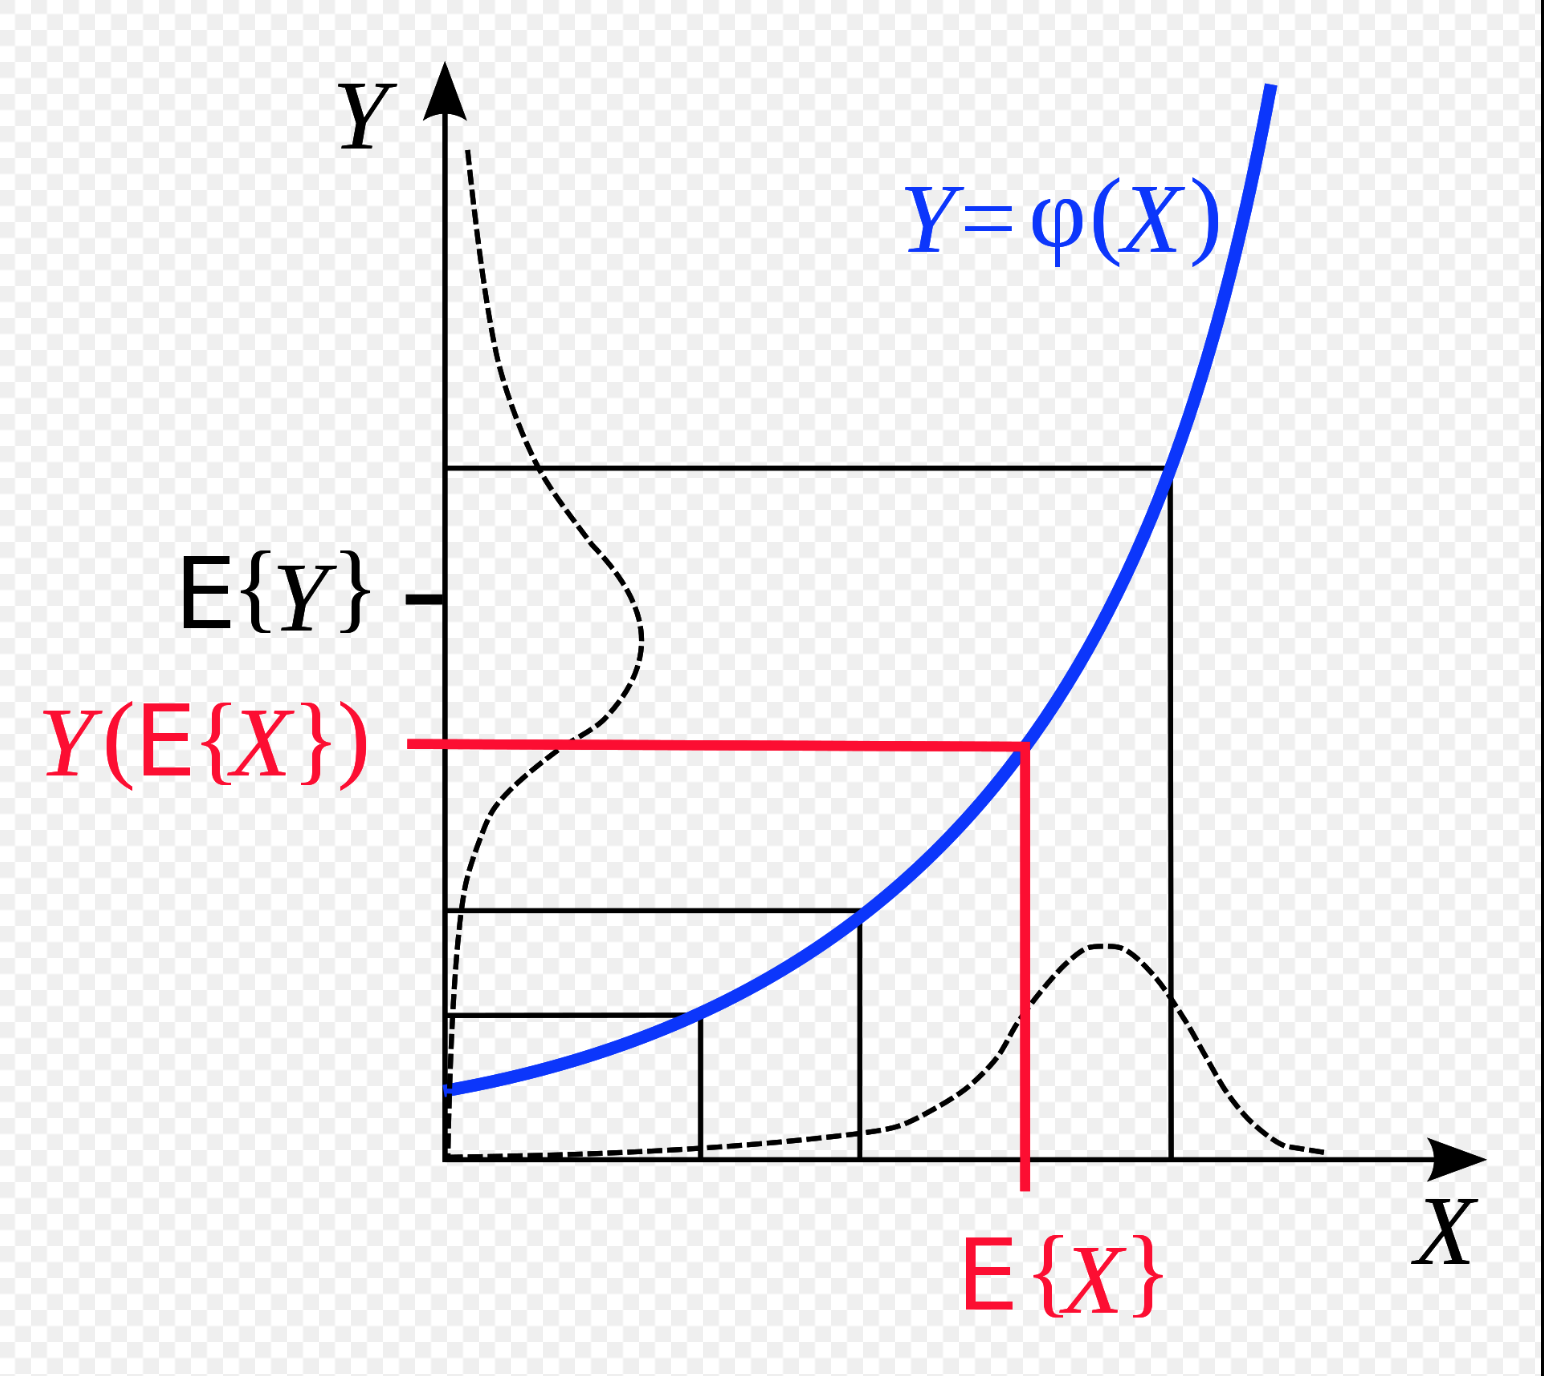
\includegraphics[width=5.0cm]{JensensInequality.png}}
\caption[fig1]{Jensen's Inequality.}
\label{fig:Jensen}
\end{figure}
